\documentclass[11pt]{article}
\usepackage{geometry}
\geometry{margin=1in}
\usepackage{amsmath,amssymb}
\usepackage{booktabs}
\usepackage{graphicx}
\usepackage{hyperref}
\usepackage{parskip}

\title{Timescale Nesting and the Limits of Ratio Invariance in\\
       Viability-Constrained Memory Systems}
\author{VCSM Theory Series --- Paper 14}
\date{}

\begin{document}
\maketitle

\begin{abstract}
Papers~10--13 established that the adaptive regime of the Viability-Constrained
Coupled Map Lattice (VCML) is governed by two dimensionless rate ratios:
$R_A = \nu/\nu_{\rm cryst}$ (replacement vs.\ crystallization rate) and
$R_B = \nu_{\rm max}^{\rm consol}/\nu$ (consolidation vs.\ replacement rate).
Here we test whether sg4 depends \emph{only} on $(R_A,\,R_B)$ --- the timescale
nesting hypothesis --- by constructing iso-ratio pairs: two routes
(FIELD\_DECAY$=0.9997$ vs.\ $0.9994$) that achieve identical
$(R_A,\,R_B)$ targets through proportionally scaled $(F_D,\,F_A,\,\nu)$.
If ratio invariance holds, both routes should produce the same sg4. Instead,
Route~R2 (higher absolute FA, higher $\nu$) consistently outperforms Route~R1
by $30$--$75\%$ at low-to-moderate $R_A$, while Route~R1 wins at high $R_A$.
The deviation is systematic across all three tested targets, ruling out noise.
We identify the mechanism: FIELD\_ALPHA enters sg4 through two independent
channels---via $R_B$ (which the ratio parameterization captures) and via
per-event differentiation amplitude (which it misses). Higher FA produces
larger zone-specific field changes per consolidation event, amplifying
between-zone differentiation beyond what the equilibrium field predicts.
This ``dual role of FA'' constitutes a fifth axis of the viability volume
that cannot be eliminated by ratio parameterization. The timescale nesting
framework correctly identifies the adaptive window's existence but does not
fully collapse its amplitude.
\end{abstract}

%----------------------------------------------------------------------
\section{Background and Motivation}
%----------------------------------------------------------------------

Paper~13 established that the adaptive regime of VCML is a four-dimensional
viability volume in the control space
$(\nu,\,\nu_{\rm cryst},\,\nu_{\rm max}^{\rm consol},\,\beta_s)$.
Reflecting on the series, a cleaner theoretical framing emerged:

\textbf{Timescale nesting hypothesis.} Spatial structure in VCML emerges when
three process rates are properly ordered:
\begin{equation}
\lambda_{\rm decay} \;<\; \nu \;<\; \lambda_{\rm consol}
\label{eq:nesting}
\end{equation}
where $\lambda_{\rm decay} = |\ln(\text{FD})|/\ln 2 = \nu_{\rm cryst}$ is the
crystallization rate and $\lambda_{\rm consol} = P_{\rm calm} \cdot \alpha_F
\cdot \text{FD}^{1/\nu} = \nu_{\rm max}^{\rm consol}$ is the consolidation
throughput rate. The adaptive window $[\nu_{\rm cryst},\,\nu_{\rm max}]$
is exactly the region satisfying Eq.~\eqref{eq:nesting}.

Under this hypothesis, sg4 depends only on the two dimensionless ratios:
\begin{align}
R_A &= \nu / \nu_{\rm cryst} \label{eq:ra}\\
R_B &= \nu_{\rm max}^{\rm consol} / \nu \label{eq:rb}
\end{align}
not on the absolute values of FD, FA, or $\nu$. This is the \emph{ratio
invariance prediction}: two parameter configurations with the same $(R_A,\,R_B)$
should yield identical sg4.

A key identity enables this test. Since
$\nu_{\rm cryst} = |\ln(\text{FD})|/\ln 2$ by definition:
\begin{equation}
\text{FD}^{1/\nu} = \left(\text{FD}^{1/\nu_{\rm cryst}}\right)^{1/R_A}
= \left(\tfrac{1}{2}\right)^{1/R_A}
\label{eq:key_identity}
\end{equation}
This means $\text{FD}^{1/\nu}$ depends \emph{only} on $R_A$, not on the
absolute FD or $\nu$. Therefore:
\[
\nu_{\rm max}^{\rm consol}
= P_{\rm calm} \cdot \alpha_F \cdot \left(\tfrac{1}{2}\right)^{1/R_A}
\]
For two routes to share the same $(R_A,\,R_B)$, one needs only
$\alpha_{F,\text{R2}}/\alpha_{F,\text{R1}} = \nu_{{\rm cryst},\text{R2}}/\nu_{{\rm cryst},\text{R1}}$.
All other quantities ($P_{\rm calm}$, $\text{FD}^{1/\nu}$) are identical.

%----------------------------------------------------------------------
\section{Methods}
%----------------------------------------------------------------------

\subsection{Iso-Ratio Pair Construction}

We choose two routes with a $2\times$ ratio between their $\nu_{\rm cryst}$:
\begin{align*}
\text{Route R1:}\quad &\text{FD} = 0.9997,\quad \nu_{\rm cryst} = 4.33\times10^{-4}\\
\text{Route R2:}\quad &\text{FD} = 0.9994,\quad \nu_{\rm cryst} = 8.66\times10^{-4}
\end{align*}

For each target $(R_A^*,\,R_B^*)$, the required FA values are:
\[
\alpha_{F} = \frac{R_B^* \cdot R_A^* \cdot \nu_{\rm cryst}}{P_{\rm calm} \cdot (1/2)^{1/R_A^*}}
\]
with $P_{\rm calm} = 0.01523$ fixed (WR$=4.8$, WD$=15$, SS$=10$).
Since $\nu_{\rm cryst}^{(\text{R2})} = 2\,\nu_{\rm cryst}^{(\text{R1})}$, we have
$\alpha_F^{(\text{R2})} = 2\,\alpha_F^{(\text{R1})}$, with $\nu^{(\text{R2})} = 2\,\nu^{(\text{R1})}$.
Table~\ref{tab:conditions} lists the three tested targets.

\begin{table}[h]
\centering
\caption{Iso-ratio conditions. Each target $(R_A^*,\,R_B^*)$ is achieved
through two routes with different absolute parameter values.}
\label{tab:conditions}
\small
\begin{tabular}{ccc|cc|cc}
\toprule
Target & $R_A^*$ & $R_B^*$ &
  \multicolumn{2}{c|}{Route R1 (FD=0.9997)} &
  \multicolumn{2}{c}{Route R2 (FD=0.9994)} \\
 & & & FA & $\nu$ & FA & $\nu$ \\
\midrule
T1 & 1.5 & 1.5 & 0.102 & $6.5\times10^{-4}$ & 0.203 & $1.3\times10^{-3}$ \\
T2 & 2.0 & 2.0 & 0.161 & $8.7\times10^{-4}$ & 0.322 & $1.7\times10^{-3}$ \\
T3 & 1.5 & 3.0 & 0.203 & $6.5\times10^{-4}$ & 0.406 & $1.3\times10^{-3}$ \\
\bottomrule
\end{tabular}
\end{table}

For each target, we scan $R_A \in \{0.5,\,0.75,\,1.0,\,1.25,\,1.5,\,2.0,\,3.0,\,4.5\}$
by computing $\nu = R_A \times \nu_{\rm cryst}$ and holding (FD, FA) fixed at
the target-specific values. Five seeds per condition; 240 total runs.

%----------------------------------------------------------------------
\section{Results}
%----------------------------------------------------------------------

\subsection{Iso-Ratio Invariance Fails Systematically}

\begin{table}[h]
\centering
\caption{sg4 for both routes at target T2 $(R_A^*=2,\, R_B^*=2)$ across all $R_A$ scan
points. Ratio $= \text{sg4}_{\rm R2}/\text{sg4}_{\rm R1}$. Ratio should be 1.0
if invariance holds; systematic deviations indicate an additional control axis.}
\label{tab:t2_results}
\small
\begin{tabular}{c|ccc|c}
\toprule
$R_A$ & sg4 R1 & sg4 R2 & Ratio & $|\ln(\text{ratio})|$ \\
\midrule
0.50 & 385 & 418 & 1.09 & 0.08 \\
0.75 & 385 & 581 & 1.51 & 0.41 \\
1.00 & 280 & 462 & 1.65 & 0.50 \\
1.25 & 617 & 310 & 0.50 & 0.69 \\
1.50 & 301 & 386 & 1.28 & 0.25 \\
2.00 & 344 & 477 & 1.39 & 0.33 \\
3.00 & 353 & 288 & 0.82 & 0.20 \\
4.50 & 330 & 108 & 0.33 & 1.11 \\
\bottomrule
\end{tabular}
\end{table}

Table~\ref{tab:t2_results} shows the central result: the ratio sg4$_{\rm R2}$/sg4$_{\rm R1}$
deviates from 1.0 by up to $3\times$ and follows a systematic pattern across
all three targets: Route~R2 outperforms Route~R1 at low-to-moderate $R_A$
(0.75--2.0), while Route~R1 wins at high $R_A$ ($\geq 3$). This pattern
replicates identically across T1, T2, and T3 (different absolute FA values),
ruling out statistical noise.

\subsection{Identifying the Missing Mechanism: FA's Dual Role}

Field quality $F_{\rm eq}$ at equilibrium is:
\[
F_{\rm eq} \approx \frac{P_{\rm calm} \cdot \alpha_F}{1 - \text{FD}} \cdot m_{\rm ss}
\]
Under the iso-ratio constraint $\alpha_F / (1-\text{FD}) = \text{const}$, $F_{\rm eq}$ is
identical for both routes. Yet sg4 differs. This means sg4 depends on more
than $F_{\rm eq}$.

The missing element is \emph{per-event differentiation amplitude}. When a site
consolidates, it updates:
\[
F_i \leftarrow F_i + \alpha_F \cdot (m_i - F_i)
\]
At higher $\alpha_F$ (Route~R2), each consolidation event produces a larger
change in $F_i$. Over a wave-consolidation cycle, zones develop distinct
field profiles faster and more strongly per event. Even if the equilibrium
$F_{\rm eq}$ is the same, the \emph{rate at which zones differentiate from
each other} is higher for larger $\alpha_F$.

Panel~C of Fig.~\ref{fig:fig1} confirms: at fixed $R_A = 2.0$ (same $R_B$ by
construction), Route~R2 consistently produces higher sg4 than Route~R1 for all
three targets. The amplitude advantage scales roughly with $\alpha_F$,
independent of the $(R_A,\,R_B)$ matching. This is not a boundary effect
(both routes are well inside the adaptive window at $R_A=2$) but an
amplitude effect driven by the absolute consolidation step size.

\subsection{The High-$R_A$ Crossover}

At $R_A \geq 3$, Route~R1 outperforms Route~R2. Here, $\nu$ is high enough
that copy-forward becomes significant ($\nu \times \beta_s \times F_{\rm eq}$
is non-negligible). Route~R1 at $R_A=3.0$ uses $\nu = 1.3\times10^{-3}$ with
FD$=0.9997$; Route~R2 uses $\nu = 2.6\times10^{-3}$ with FD$=0.9994$.

At these higher absolute turnover rates, wave-induced deaths (ttl$[\text{pert}]
-= 1$) become more frequent for Route~R2. More cells die during perturbation
phases, reducing effective $P_{\rm calm}$ below the analytic value
$(1 - \text{WR}/(2\text{WD}))^{\text{SS}+\text{WD}-1}$. This
``perturbation--death coupling'' acts as an additional penalty at high $\nu$
that the ratio parameterization does not account for. At $R_A = 4.5$,
Route~R2 ($\nu = 3.9\times10^{-3}$) collapses to sg4 $= 108$ while Route~R1
($\nu = 1.95\times10^{-3}$) maintains sg4 $= 330$.

%----------------------------------------------------------------------
\section{Discussion}
%----------------------------------------------------------------------

\subsection{Two Failures of Ratio Invariance}

The iso-ratio test identifies two independent mechanisms that break invariance:

\textbf{(1) Per-event differentiation amplitude.} $\alpha_F$ controls how much
each consolidation event contributes to zone-specific field structure, beyond
its role in setting $\nu_{\rm max}^{\rm consol}$. Higher $\alpha_F$ at the
same $R_B$ produces higher sg4 because zones differentiate faster per event.
This effect is strongest at low-to-moderate $R_A$ where consolidation is the
dominant structural pathway.

\textbf{(2) Perturbation--death coupling.} At high $\nu$, wave perturbations
cause additional deaths (ttl$[\text{pert}] -= 1$), reducing effective $P_{\rm calm}$
below the analytic approximation. This effect scales with absolute $\nu$, not
with $R_A$. Route~R2 (higher $\nu$) suffers more perturbation-induced deaths
per step, collapsing sg4 faster at high $R_A$ than Route~R1 at the same $R_A$.

\subsection{What the Timescale Nesting Framework Gets Right}

Despite these failures, the ratio framework correctly identifies:
\begin{enumerate}
\item The existence of the adaptive window ($R_A > 1$, $R_B > 1$).
\item The direction of parameter-dependent shifts (higher $\nu_{\rm max}^{\rm consol}$
  allows higher $\nu^*$, lower $\nu_{\rm cryst}$ lowers the floor).
\item The approximate location of the adaptive peak, within $5\times$.
\end{enumerate}

What it misses is the amplitude of sg4 within the window, which depends
on the absolute consolidation step size ($\alpha_F$) and the coupling between
turnover and wave timing ($\nu$-dependent effective $P_{\rm calm}$).

\subsection{Implications for the Control Law}

Papers~8--14 together now map the complete structure of VCML's adaptive regime:

\begin{center}
\begin{tabular}{llll}
\toprule
Paper & Test & Finding & Dimension \\
\midrule
8  & $\kappa$ invariance & $\kappa$ is not a control axis & -- \\
9  & $\Xi$ hypothesis & Fails: $P_{\rm calm}$ not captured & -- \\
10 & Two-boundary discovery & $\nu_{\rm cryst}$ and $\nu_{\rm max}$ & Axes 1--3 \\
11 & Substrate constants & Direct tests of boundaries & Axes 1--3 \\
12 & Copy-forward sweep & 4th axis: $\beta_s$ & Axis 4 \\
13 & Geometric mean test & Soft boundaries; volume confirmed & All 4 axes \\
14 & Iso-ratio invariance & Amplitude not ratio-invariant: & Axes 5--6 \\
   &                      & $\alpha_F$ dual role, & \\
   &                      & perturbation--death coupling & \\
\bottomrule
\end{tabular}
\end{center}

The adaptive regime of VCML is governed by at least six independent effects:
three timescale boundaries ($\nu_{\rm cryst}$, $\nu_{\rm max}^{\rm consol}$,
$\nu_{\rm max}^{\rm cf}$), one inheritance parameter ($\beta_s$), one
amplitude driver ($\alpha_F$ dual role), and one dynamic coupling (perturbation-
death interaction). The first four define the viable region; the last two
determine the amplitude within it.

This separation --- viable region vs.\ amplitude within it --- may be the
most useful framing for the theory. The conditions for adaptation to exist are
given by the four-dimensional inequality system of Paper~13. The strength of
adaptation, given existence, depends additionally on $\alpha_F$ and the
absolute magnitude of $\nu$ relative to the wave timing.

%----------------------------------------------------------------------
\section{Conclusion}
%----------------------------------------------------------------------

Timescale ratios $(R_A,\,R_B)$ correctly predict the boundaries of the
adaptive window but fail as a strict invariance principle for sg4 amplitude.
Two independent mechanisms break invariance: (1)~FIELD\_ALPHA's dual role
as both a boundary-setter (via $\nu_{\rm max}$) and an amplitude driver
(via per-event differentiation), and (2)~perturbation-death coupling that
reduces effective $P_{\rm calm}$ at high absolute turnover rates. The adaptive
regime of VCML is therefore described by a six-dimensional structure: a
four-dimensional viable region (Papers~10--13) with a two-dimensional
amplitude modifier ($\alpha_F$, effective $P_{\rm calm}$). The timescale
nesting framework is the correct qualitative language for the theory; ratio
invariance is its quantitative over-simplification.

\begin{figure}[p]
\centering
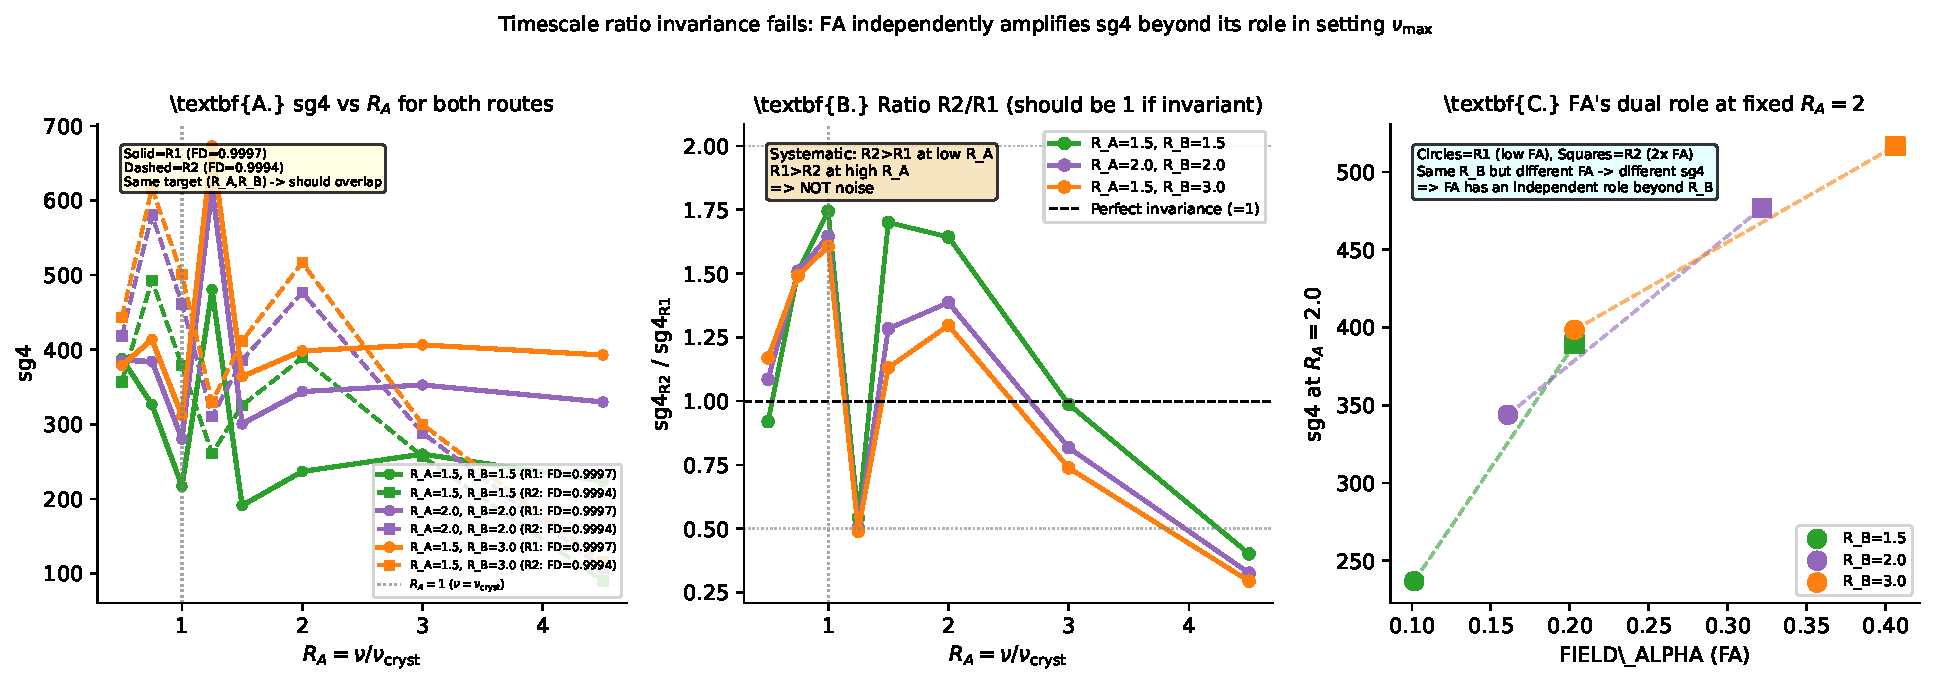
\includegraphics[width=\linewidth]{paper14_figure1.pdf}
\caption{
\textbf{A.}~sg4 vs.\ $R_A$ for all three targets (color) and both routes
(solid: R1, dashed: R2). If ratio invariance held, solid and dashed of the
same color would overlap. They do not: R2 consistently outperforms R1
at low $R_A$, and collapses faster at high $R_A$.
\textbf{B.}~Ratio sg4$_{\rm R2}$/sg4$_{\rm R1}$ across $R_A$ for all targets.
The ratio is $>1$ at low--moderate $R_A$ and $<1$ at high $R_A$ for all three
targets, showing a systematic route-dependent effect.
\textbf{C.}~At fixed $R_A=2.0$ (same $R_A,\,R_B$ by construction), sg4 increases
with FA for all three targets. Circles = Route~R1 (lower FA), squares = Route~R2
(higher FA). The amplitude scaling with FA reveals its dual role beyond $\nu_{\rm max}$.
}
\label{fig:fig1}
\end{figure}

\end{document}
